\documentclass[a4paper,12pt]{article}
\usepackage[ngerman]{babel}
\usepackage{ucs}
\usepackage{multirow}
\usepackage{xltxtra}
\usepackage[utf8x]{inputenc}
\usepackage{fontspec}
\usepackage[automark]{scrpage2}
\usepackage{eurosym}
\usepackage{graphicx}
\usepackage[paper=a4paper,left=25mm,right=25mm,top=25mm,bottom=25mm]{geometry}
\pagestyle{scrheadings}
\setmainfont[Mapping=tex-text]{Liberation Serif}
\clearscrheadfoot
\begin{document}
\ohead{Regelstand: \today}
\title{Regeln Linefollowing Challenge 2018}

 \begin{center}

\includegraphics[width=0.5\textwidth]{logo.png}

\huge                      % Schriftgröße einstellen
\bfseries                   % Fettdruck einschalten
Regeln Linefollowing Challenge 2018
  \end{center}
  %Inhaltliche Änderungen im Vergleich zu den Regeln von 2017 sind \textbf{fett} markiert. Im Zweifel ist die Interpretation der Regeln durch die Schiedsrichter bindend.
\section{Aufgabe}
Baue und programmiere einen Linienfolger-Roboter, der einer schwarzen Linie auf weißem Untergrund zu
einem Karton folgen kann und zunächst mindestens einen Ball dorthin liefert und dann zum Start zurückkehrt.
Anschließend kann er in der verbleibenden Zeit (3 Minuten) zum Karton zurückkehren (so oft wie nötig) um
eine für jede Altersgruppe \emph{festgelegte} Zahl an Bällen (nicht mehr und nicht weniger) zum Karton zu liefern.
\section{Wer kann teilnehmen?}
Teams von \emph{2 bis 4 Spielern} in \emph{folgenden Altersgruppen}:
\begin{itemize}
		\item Altersgruppe MS: 10-13 Jahre
		\item Altersgruppe HS: 14-17 Jahre
		\item Altersgruppe UP: 18-20 Jahre
\end{itemize}
\section{Materialanforderungen}
Ein autonomer Roboter basierend auf jeglicher Plattform der maximal \euro{1500} kostet und die folgenden
Designanforderungen erfüllt, welche während des Check-Ins am ersten Wettbewerbstag überprüft werden:

\begin{itemize}
	\item Der Roboter muss zeigen, dass er ein Linienfolgerprogramm benutzt, indem er die letzten 60 cm der
	diesjährigen Strecke abfährt (Wenn in den letzten 60 cm eine Abzweigung ist, startet der Roboter direkt hinter
	dieser Abzweigung)
	\item Der Roboter muss zeigen, dass er vor dem Turm anhält (er muss nicht zeigen, dass er Bälle liefern oder sich
	umdrehen kann)
	\item Das Volumen des Roboters darf 65030 cm3 nicht überschreiten.
	\item Mehrere Sensoren und Prozessoren sind erlaubt.
\end{itemize}
\section{Spielregeln}
\begin{itemize}
	\item Ein Linienfolger-Programm muss die Bewegung des Roboters steuern
	\item Der Roboter muss die Aufgabe innerhalb von 3 Minuten bewältigen
	\item Nur Spieler dürfen während dem Durchlauf den Roboter berühren, keine Coaches
	\item Der \emph{Karton} darf nicht von Personen berührt werden
	\item \textbf{Ebenso ist es nicht erlaubt die Bewegung der Bälle aus dem Karton manuell
	zu beschleunigen.}
	\item \textbf{Wenn ein Spieler den Karton berührt oder in den Karton greift, erhält das Team lediglich
	400 Punkte für die Strecke egal wie viele Bälle geliefert werden.}
	\item Wenn der Roboter von einem Spieler berührt wird, muss er zurück auf den Startpunkt gesetzt werden
	\item Offizielle Strecken werden bei der Vorbereitung zur Übung bereitgestellt
\end{itemize}
\section{Spielfeld}

\emph{Die Strecke:}
\begin{itemize}
	\item Weiße PVC-Plane \textbf{oder Papier}
	\item Altersgruppe 1 – Eine Abzweigung, 1,3 cm dicke schwarze Linie
	\item Altersgruppen 2 \& 3 – Zwei Abzweigungen, 0,75 cm dicke schwarze Linie
	\item \textbf{Vor dem Karton befindet sich eine gerade Strecke von mindestens 20 cm.}
	\item \textbf{Die Linie zur Markierung der Strecke befindet sich nie näher als 10 cm
	an einer anderen Linie oder der Kante des Plans.}
	\item \textbf{Anderer Text auf dem Plan befindet sich immer mindestens 10 cm von der Linie
	entfernt}
	\item \textbf{Die Kurven können sich im Radius unterscheiden, aber keine Kurve darf einen
	Radius kleiner als 15 cm für die Altersgruppe MS oder 10 cm für die Altersgruppen HS und UP haben.}
	\item \textbf{Das Licht am Ort der Strecke kann sich über die Tageszeit ändern. Teams müssen
	auf diese Bedingungen vorbereitet sein.}
	\item \textbf{Die Altersgruppe MS und HS haben jeweils eine eigene Strecke. Ob für die
	Altersgruppe UP die HS-Strecke oder eine eigens dafür erstellte verwendet wird obliegt der
	Entscheidung der Schiesrichter.}
	\item \textbf{ Die Schiedsrichter können entscheiden die Öffnung des Kartons für die
	Altersgruppe UP zu verkleinern.}
\end{itemize}
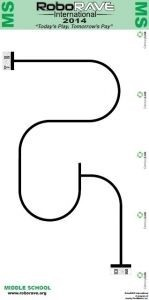
\includegraphics[width=0.3\textwidth]{track_ms_lf.png}
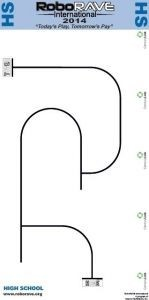
\includegraphics[width=0.3\textwidth]{track_hs_lf.png}

\emph{Der Karton:}
\begin{itemize}
\item Alle Altersgruppen benutzen denselben Karton , der ungefähr 20 cm hoch ist und ein 10×10 cm großes Loch
an der Oberseite und eine offene Rückwand hat. Der Karton ist mit Klebeband fest am Untergrund befestigt
\item Es kann durch die Veranstalter ein Mechanismus zum Zählen der Bälle im Karton angebracht werden, der die
Bewegung der Bälle nicht behindert
\end{itemize}
\emph{Die Strecke und der Karton dürfen nicht modifiziert werden!}
\section{Wertungszeitraum}
\par Die Art der Wertung der einzelnen Ergebnisse im Bezug auf den gesamten Wettbewerb wird am ersten Wettbewerbstag von den Schiedsrichtern bekanntgegeben. Änderungen der Wertungsmodalitäten bleiben den Schiedsrichtern vorbehalten.
\section{Punktevergabe}
Die Gesamtpunktzahl ist die Summe der Punkte aus der ersten Fahrt zum Karton und den Bällen, die während
den weiteren Fahrten zum Karton geliefert werden.
\begin{itemize}
\item Jede Altersgruppe hat eine \textbf{von den Schiedsrichtern zu Beginn des Wettbewerbs festgelegte} Anzahl an Bällen, die sie zum Karton liefern muss:
\begin{itemize}
	\item Altersgruppe MS - \textbf{zwischen 125 und 200 Bällen}
\item Altersgruppe HS – \textbf{zwischen 200 und 250 Bällen}
\item Altersgruppe UP - \textbf{zwischen 100 und 350 Bällen (die Zahl ist niedrig sollten die Schiedsrichter
entscheiden die Öffnung des Kartons zu verkleinern)}
\end{itemize}
\item Wenn \emph{mehr} Bälle zum Karton geliefert wurden als die festgelegte Anzahl werden alle zusätzlichen Bälle von
der festgelegten Anzahl \emph{subtrahiert} um die Punktzahl zu erhalten. Wenn weniger oder gleich viele Bälle zum
Karton geliefert werden, ist die Anzahl der gelieferten Bälle die Punktzahl.
\item Der während der ersten Fahrt gelieferte Ball wird nicht als Bonuspunkt gezählt, sondern dient lediglich dazu
zu zeigen, dass der Roboter zum Transport von Bällen in der Lage ist. Es muss während der ersten Fahrt nur
1 Ball zum Karton geliefert werden. In der ersten Runde mehr Bälle als einen zum Karton zu liefern hat weder
positive noch negative Konsequenzen. Die Bälle von der ersten Fahrt werden vor dem Zählen entfernt.
\item Wenn der Roboter die benötigte Anzahl an Bällen vor Ablauf der 3 Minuten zum Karton geliefert hat sollte er
anhalten
In der Punktetabelle sind die Punkte für die erste Fahrt zum Karton aufgelistet.
\end{itemize}
\section{Punktetabelle}
\begin{center}
\begin{tabular}{|c|c|c|c|c|c|} \hline
	\multirow{3}*{} & Verlässt & Passiert erste & Passiert zweite & Stoppt vor dem & Liefert einen \\
	 & Startpunkt & Abzweigung & Abzweigung & Karton & Ball zum Karton \\ \hline
	10-13 (MS) & 25 & 25 & n.v. & 100 & 100 \\ \hline
	14-17 (HS) & 25 & 25 & 25 & 50 & 100 \\ \hline
	18-20 & 25 & 25 & 25 & 50 & 100 \\ \hline
\end{tabular}
\begin{tabular}{|c|c|c|c|c|c|} \hline
	\multirow{3}*{} & Startet den & Passiert erste & Passiert zweite & Kommt am & Gesamt \\
	& Rückweg & Abzweigung & Abzweigung & Startpunkt an &  \\ \hline
	10-13 (MS) & 25 & 25 & n.v. & 100 & 400 \\ \hline
	14-17 (HS) & 25 & 25 & 25 & 100 & 400 \\ \hline
	18-20 & 25 & 25 & 25 & 100 & 400 \\ \hline
\end{tabular}
\end{center}
\end{document}
